\documentclass[9pt, aspectratio=169]{beamer}
\usepackage{FiraSans}
\usetheme[subsectionpage=progressbar]{metropolis}
\usepackage[utf8]{inputenc}
\usepackage{amsmath}
\usepackage{amsfonts}
\usepackage{amssymb}
\usepackage{multicol}
\usepackage{tikz}
\usetikzlibrary{positioning, decorations, calligraphy}
\usepackage{caption}
\usepackage{xcolor}
\usepackage[T1]{fontenc} 
\usepackage[skins]{tcolorbox}
\author{Nicola Roman\`o - nicola.romano@ed.ac.uk}
\title{Lecture 18 - Autoencoders}
\setlength{\fboxsep}{0pt}
\setbeamertemplate {footline}{\begin{scriptsize}\hfill\insertframenumber ~of \inserttotalframenumber\kern1em\vskip5pt\end{scriptsize}}

% Remove "Figure" in front of captions
% See https://tex.stackexchange.com/questions/82456/how-to-remove-figure-caption-prefix-figure-in-beamer
\captionsetup{labelformat=empty,labelsep=none}

\titlegraphic{\centering \includegraphics[scale=.5]{instituteLogo.png}}
\date{}

\begin{document}

\newtcolorbox{codebox}{enhanced,
    top=2pt,
    left=2pt,
    right=2pt,
    bottom=2pt,
    boxrule=0pt,
    leftrule=5pt,
    sharp corners,
    colback=gray!20,
    colframe=blue!60!black}

\begin{frame}
    \titlepage
\end{frame}

\begin{frame}
    {Learning objectives}
    \begin{columns}
        \begin{column}{0.8\textwidth}
            \begin{itemize}
                \item Discuss autoencoders and their applications.
                \item Code a denoising autoencoder using Keras.
            \end{itemize}
        \end{column}
        \begin{column}{0.2\textwidth}
            
\includegraphics[angle=-30, origin=tr, width=1.5\textwidth]{lightbulb.png}
        \end{column}
    \end{columns}
\end{frame}

\section{Introduction}

\begin{frame}
    {What is an autoencoder?}

    \begin{itemize}
        \item An \textbf{autoencoder} is a neural network that is trained to reconstruct its input.
        \item It consists of an \textbf{encoding} part and a \textbf{decoding} part.
              \onslide<2->{
        \item The easiest mapping of an input to itself would be the identity function.
        \item Autoencoders force the input to be compressed, and then decompressed to reconstruct it.
              }
              \onslide<3->{
        \item It can only reconstruct an approximated version of the input.
              }
    \end{itemize}

    \onslide<1->
    {
        \centering
        \includegraphics[width=.35\textwidth]{Autoencoder_schema.png}

        \footnotesize
        Source: Wikipedia
    }

\end{frame}

\begin{frame}
    {Convolutional autoencoders}
    A \textbf{convolutional autoencoder} is a convolutional network that is trained to reconstruct its input.
    \vspace{2em}

    \centering
    \begin{tikzpicture}
        % Input image
        \node (input) [text width=2cm, text height=2cm] at (0,0) {\includegraphics[width=\textwidth]{HnE.png}};

        % Conv layers
        \foreach \x [count=\N] in {3,3.5,...,4.5}
            {
                \node (layer\N) [draw, rectangle, fill=orange!50!yellow, minimum width=0.3cm, minimum height=2cm - \N * 0.3 cm] at (\x,0) {};
            }
        \node (layer5) [draw, rectangle, fill=green!30!yellow, minimum width=0.3cm, minimum height=0.5cm] at (5,0) {};

        \foreach \x [count=\N from 6] in {5.5,6,...,7}
            {
                \pgfmathsetmacro{\Nn}{(10 - \N)*0.3}
                \node (layer\N) [draw, rectangle, fill=orange!50!yellow, minimum width=0.3cm, minimum height=2cm - \Nn cm] at (\x,0) {};
            }

        \node (output) [text width=2cm, text height=2cm] at (10,0) {\includegraphics[width=\textwidth]{HnE_out.png}};

        % Labels
        \node [below =of input, yshift=1cm] {\Large$X$};
        \node [below =of output, yshift=1cm] {\Large$X'$};
        \node at (5, -3) {\Large$X\simeq X'$};
        \node (latent-label) [color=green!30!yellow!60!black, text width=7em, align=center] at (5, -1.5) {\mbox{Latent space} (bottleneck)};
        \draw [decorate,
            decoration = {calligraphic brace, amplitude=5pt, raise=0.5em}, thick] (3, 1) -- (4.5, 1) node [above, align=center, anchor=south east, yshift=1em] {Encoder};
        \draw [decorate,
            decoration = {calligraphic brace, amplitude=5pt, raise=0.5em}, thick] (5.5, 1) -- (7, 1) node [above, align=center, anchor=south east, yshift=1em] {Decoder};

        % Arrows
        \draw [->] (input) -- (layer1.west);
        \foreach \N [count=\Nn from 2] in {1,2,...,8}
            {
                \draw [->] (layer\N) -- (layer\Nn.west);
            }
        \draw [->] (layer9.east) -- (output);
        \draw [->, color=green!30!yellow!60!black] (latent-label) -- (layer5);
    \end{tikzpicture}

    \pause
    While ideally the input is identical to the output, in practice we get a slightly degraded version.

    \centering
    \textbf{Why would we do this?}
\end{frame}

\begin{frame}
    {Uses of autoencoders}
    Autoencoders have been used in a variety of applications, including image analysis.

    Examples of uses in computer vision include
    \begin{itemize}
        \item Noise reduction
        \item Image colorization
        \item Image compression
        \item Image restoration
        \item Superresolution
    \end{itemize}

    Outside of computer vision, autoencoders are used in a variety of applications, including fraud detection, recommendation systems, and text translation.
\end{frame}

\begin{frame}
    {Building an autoencoder in Keras}
    We will now build a  simple autoencoder that just learns to reconstruct its input (trained on Fashion MNIST).

    \centering
    See \texttt{basic\_autoencoder.ipynb}

    \begin{tikzpicture}
        % Input image
        \node (input) [text width=2cm, text height=2cm] at (0,0) {\includegraphics[width=\textwidth]{FashionMNIST.png}};

        % Conv layers
        \foreach \x [count=\N] in {3,3.5,...,4.5}
            {
                \node (layer\N) [draw, rectangle, fill=orange!50!yellow, minimum width=0.3cm, minimum height=2cm - \N * 0.3 cm] at (\x,0) {};
            }
        \node (layer5) [draw, rectangle, fill=green!30!yellow, minimum width=0.3cm, minimum height=0.5cm] at (5,0) {};

        \foreach \x [count=\N from 6] in {5.5,6,...,7}
            {
                \pgfmathsetmacro{\Nn}{(10 - \N)*0.3}
                \node (layer\N) [draw, rectangle, fill=orange!50!yellow, minimum width=0.3cm, minimum height=2cm - \Nn cm] at (\x,0) {};
            }

        \node (output) [text width=2cm, text height=2cm] at (10,0) {\includegraphics[width=\textwidth]{FashionMNIST.png}};

        % Arrows
        \draw [->] (input) -- (layer1.west);
        \foreach \N [count=\Nn from 2] in {1,2,...,8}
            {
                \draw [->] (layer\N) -- (layer\Nn.west);
            }
        \draw [->] (layer9.east) -- (output);
    \end{tikzpicture}

\end{frame}

\section {Uses of autoencoders}
\subsection {Compression}

\begin{frame}
    {Autoencoders as compressors}
    \begin{itemize}
        \item The \textbf{latent space} is a low-dimensional representation of the input.
              \pause
        \item We can use it to compress the input.
              \pause
        \item Useful e.g. to reduce the size of images/videos for display purposes (e.g. streaming a video).
    \end{itemize}

    \centering
    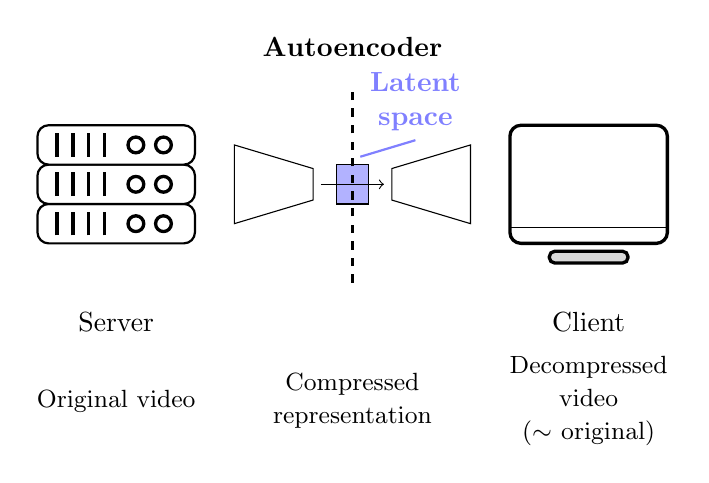
\begin{tikzpicture}
        % Server
        \foreach \y in {0.25, 0.75, 1.25}
            {
                \node [draw, rectangle, rounded corners, thick, fill=white, minimum width=2cm, minimum height=0.5cm] at (0,\y) {};
                \foreach \x in {-0.75, -0.55, ..., 0}
                    {
                        \draw [very thick] (\x, \y - 0.15) -- (\x, \y + 0.15);
                    }
                \draw [very thick] (0.25, \y) circle (0.1);
                \draw [very thick] (0.6, \y) circle (0.1);
            }

        % Encoder
        \draw [fill=white] (1.5, 0.25) -- (1.5, 1.25) -- (2.5, 0.95) -- (2.5, 0.55) -- cycle;

        % Latent space
        \draw [fill=blue!30!white] (2.8, 1) rectangle (3.2, 0.5);

        % Separator
        \draw [very thick, color=black, dashed] (3, -0.5) -- (3, 2);

        % Decoder
        \draw [fill=white] (4.5, 0.25) -- (4.5, 1.25) -- (3.5, 0.95) -- (3.5, 0.55) -- cycle;


        % Arrows
        \draw [->] (2.6, 0.75) -- (3.4, 0.75);

        % Client
        \draw [very thick, fill=white, rounded corners] (5, 0) rectangle (7, 1.5);
        \draw (5, 0.2) -- (7, 0.2);
        \draw [very thick, fill=gray!30!white, rounded corners=0.07cm] (5.5, -0.1) rectangle (6.5, -0.25);

        % Labels
        \node at (0, -1) {Server};
        \node at (6, -1) {Client};
        \node at (0, -2) {\small Original video};
        \node [text width=6em, align=center] at (3, -2) {\small Compressed \mbox{representation}};
        \node [text width=6em, align=center] at (6, -2) {\small Decompressed video \mbox{($\sim$ original)}};
        \node at (3, 2.5) {\textbf{Autoencoder}};
        \node (latent) [color=blue!50!white, text width = 5em, align=center] at (3.8, 1.8) {\textbf{Latent space}};
        \draw [color=blue!50!white, thick] (latent.south) -- (3.1, 1.1);
    \end{tikzpicture}
\end{frame}

\begin{frame}
    {Autoencoders for feature extraction}
    We can think of the latent space as an \textit{optimal} low-dimensional representation of the input, therefore we can use it to generate features from the input.

    \pause
    Example:
    \centering
    \includegraphics[width=\textwidth]{paco ramos.png}
\end{frame}

\begin{frame}
    {Classification of leaves using autoencoders}
    \centering
    \includegraphics[height=.9\textheight]{paco ramos 2019 method.png}
\end{frame}

\subsection{Denoising}

\begin{frame}
    {Autoencoders for denoising}
    \begin{itemize}
        \item Noisy image = original image + noise
        \item Since the autoencoder learns only the \textit{important} features of the image, it will not learn random noise.
        \item We can \textit{trick} the autoencoder by feeding it pairs of noisy/clean images as source and target, and it will learn to denoise the images!
    \end{itemize}


    \centering
    \begin{tikzpicture}
        % Input image
        \node (input) [text width=2cm, text height=2cm] at (0,0) {\includegraphics[width=\textwidth]{HnEnoise.png}};

        % Conv layers
        \foreach \x [count=\N] in {3,3.5,...,4.5}
            {
                \node (layer\N) [draw, rectangle, fill=orange!50!yellow, minimum width=0.3cm, minimum height=2cm - \N * 0.3 cm] at (\x,0) {};
            }
        \node (layer5) [draw, rectangle, fill=green!30!yellow, minimum width=0.3cm, minimum height=0.5cm] at (5,0) {};

        \foreach \x [count=\N from 6] in {5.5,6,...,7}
            {
                \pgfmathsetmacro{\Nn}{(10 - \N)*0.3}
                \node (layer\N) [draw, rectangle, fill=orange!50!yellow, minimum width=0.3cm, minimum height=2cm - \Nn cm] at (\x,0) {};
            }

        \node (output) [text width=2cm, text height=2cm] at (10,0) {\includegraphics[width=\textwidth]{HnE.png}};

        % Labels
        \node [below =of input, yshift=1cm] {\Large X + noise};
        \node [below =of output, yshift=1cm] {\Large X};

        % Arrows
        \draw [->] (input) -- (layer1.west);
        \foreach \N [count=\Nn from 2] in {1,2,...,8}
            {
                \draw [->] (layer\N) -- (layer\Nn.west);
            }
        \draw [->] (layer9.east) -- (output);
    \end{tikzpicture}
\end{frame}

\begin{frame}
    {Denoising using an autoencoder}
    Let's update our code to make a denoising autoencoder!

    \centering
    See \texttt{denoising\_autoencoder.ipynb}
    \begin{tikzpicture}
        % Input image
        \node (input) [text width=2cm, text height=2cm] at (0,0) {\includegraphics[width=\textwidth]{FashionMNISTnoise.png}};

        % Conv layers
        \foreach \x [count=\N] in {3,3.5,...,4.5}
            {
                \node (layer\N) [draw, rectangle, fill=orange!50!yellow, minimum width=0.3cm, minimum height=2cm - \N * 0.3 cm] at (\x,0) {};
            }
        \node (layer5) [draw, rectangle, fill=green!30!yellow, minimum width=0.3cm, minimum height=0.5cm] at (5,0) {};

        \foreach \x [count=\N from 6] in {5.5,6,...,7}
            {
                \pgfmathsetmacro{\Nn}{(10 - \N)*0.3}
                \node (layer\N) [draw, rectangle, fill=orange!50!yellow, minimum width=0.3cm, minimum height=2cm - \Nn cm] at (\x,0) {};
            }

        \node (output) [text width=2cm, text height=2cm] at (10,0) {\includegraphics[width=\textwidth]{FashionMNIST.png}};

        % Arrows
        \draw [->] (input) -- (layer1.west);
        \foreach \N [count=\Nn from 2] in {1,2,...,8}
            {
                \draw [->] (layer\N) -- (layer\Nn.west);
            }
        \draw [->] (layer9.east) -- (output);
    \end{tikzpicture}
\end{frame}

\subsection{Domain adaptation}

\begin{frame}
    {Domain adaptation}
    \textbf{Domain adaptation} is an approach to transfer knowledge from one domain to another.

    \centering
    \only<1>
    {
        \includegraphics[width=.6\textwidth]{Choudhary_2020_domain_adaptation.png}

        \footnotesize
        Choudary et al. 2020.
    }
    \only<2>
    {
        \includegraphics[width=\textwidth]{Choudhary_2020_examples.png}

        \footnotesize
        \raggedright
        Choudary et al. 2020.
    }
\end{frame}
\end{document}

